\documentclass[11pt,a4paper]{article}
\usepackage[T1]{fontenc}
\usepackage[utf8]{inputenc}
\usepackage{lmodern,microtype}
\usepackage[margin=25mm,top=23mm,bottom=23mm,headheight=14pt]{geometry}
\usepackage{amsmath,amssymb,amsthm,mathtools,booktabs,array,enumitem,listings,xcolor,fancyhdr,tabularx,xurl,tikz}
\definecolor{ink}{HTML}{143549}
\definecolor{accent}{HTML}{136466}
\definecolor{quiet}{HTML}{4C5E65}
\usepackage[hypertexnames=false,colorlinks=true,linkcolor=accent,citecolor=accent,urlcolor=accent,pdfauthor={},pdftitle={Degree multiplicity and distance in Graffiti graphs}]{hyperref}
\newtheorem{theorem}{Theorem}[section]
\newtheorem{lemma}[theorem]{Lemma}
\newtheorem{proposition}[theorem]{Proposition}
\newtheorem{corollary}[theorem]{Corollary}
\theoremstyle{remark}\newtheorem*{remark}{Remark}
\newcommand{\ad}{\operatorname{ad}}
\newcommand{\diam}{\operatorname{diam}}
\newcommand{\rad}{\operatorname{rad}}
\newcommand{\supp}{\operatorname{supp}}
\DeclareMathOperator{\dist}{dist}
\newcommand{\dd}{\mathrm d}
\newcommand{\cH}{\mathcal H}
\newcommand{\doi}[1]{\href{https://doi.org/#1}{doi: #1}}
\setlist{topsep=4pt,itemsep=2pt,parsep=0pt}
\lstset{basicstyle=\ttfamily\footnotesize,columns=fullflexible,keepspaces=true,showstringspaces=false,breaklines=true,aboveskip=6pt,belowskip=6pt,frame=single,rulecolor=\color{quiet!30},xleftmargin=4pt,xrightmargin=4pt,framesep=4pt}
\pagestyle{fancy}\fancyhf{}\fancyhead[L]{\small\color{quiet}Degree multiplicity and distance in Graffiti graphs}
\fancyfoot[C]{\thepage}
\renewcommand{\headrulewidth}{0.3pt}
\setlength{\parindent}{1.2em}
\setlength{\emergencystretch}{2em}
\raggedbottom
\begin{document}\thispagestyle{plain}
\noindent{\small\sffamily\bfseries\color{accent} EXTREMAL GRAPH THEORY}\par
\vspace{6pt}
\noindent{\LARGE\bfseries\color{ink} Degree multiplicity and distance in Graffiti graphs}\par
\vspace{4pt}
\noindent{\large Inverse degrees, modal distances and coordinates of maximal independent sets}\par
\vspace{7pt}\noindent{\small Research manuscript \quad 21 November 2026}\par
\vspace{8pt}\hrule\vspace{8pt}
\noindent\textbf{Abstract.} Item 3 of Fajtlowicz's 1988 list asks whether the sum of reciprocal degrees is at most the Randi\'c index plus the maximum number of vertices sharing a degree. A 34-vertex connected bipartite graph violates the inequality. On $n$ vertices the maximum ratio of its two sides is $\frac13\log n-\frac23\log\log n+O(1)$. This asymptotic persists, up to bounded error, on graphs where the unique distance mode is the diameter and the mean distance is an arbitrarily small fraction of it. We answer the all-maximal-independent-set question in catalogue entry 90 and identify $5/4$ as the sharp multiplicative correction up to additive error. A unicyclic graph of girth five refutes entry 118R, and the corresponding sharp multiplier on each fixed-girth unicyclic class is two. Distance variance and temperature estimates give affirmative results for entries 87, 171 and 217. We also determine the order of simultaneous violations of five degree- and distance-based bounds and reproduce proofs of the original radius and mean-distance inequalities used here.

\section{The questions and their numbering}\label{sec:questions}
All graphs are finite, simple and undirected. Distance questions concern connected graphs of order $n\ge2$. Write $d_v$ for vertex degree, $D$ for diameter, $r$ for vertex radius, $m$ for the most frequent distance between distinct unordered vertices, and $\mu$ for their mean distance. In a tie use the largest modal distance, as in the 1988 paper \cite{faj}. Write $\nu$ for the matching number. The indices used below are
\[
 J=\sum_v\frac1{d_v},\qquad F=\max_j|\{v:d_v=j\}|,\qquad
 M=\sum_{uv\in E}\frac1{\max(d_u,d_v)},\quad R=\sum_{uv\in E}\frac1{\sqrt{d_ud_v}}.
\]
We also use $H=\sum_{uv\in E}2/(d_u+d_v)$ and $M\le H\le R$. The original numbering in the first table is that of the list headed \emph{Open} on p.~115 of the 1988 article. The abbreviation WoW denotes the later \emph{Written on the Wall} catalogue \cite{wow}.

\smallskip\noindent\begin{tabularx}{\linewidth}{@{}r l X@{}}\toprule
1988 & Proposed inequality & Result and proof in this paper\\\midrule
3 & $J\le R+F$ & False. Section~\ref{sec:degree-data} gives the certificate and optimal growth rate.\\
5 & $m\le\mu+R$ & False. Sections~\ref{sec:joint} and~\ref{sec:finitecert} give joint and finite examples.\\
11 & $r\le\mu+R$ & True. It follows from item 12 and $\mu\ge1$.\\
12 & $r\le1+R$ & True. Appendix~\ref{sec:radius-certified} bounds $R-r$ with a sharp path exception.\\
13 & $\mu\le R$ & True. Appendix~\ref{sec:mass} proves it by optimizing and deleting vertex mass.\\\bottomrule
\end{tabularx}

\medskip\noindent The proofs of 11--13 build on VMRC manuscripts [161], [171], [226] and [227] \cite{cat-rad,cat-harm,audited,mass-audit}. The finite certificate for item 5 appeared in the preceding distance-mode manuscript \cite{earlier-modes}. The present paper supplies item 3 in full and uses nested neighborhoods inside the distance construction to reach both extremal regimes simultaneously. Different methods operate on different graphs: the bipartite examples control degree multiplicities, the maximal-independent-set arguments count neighbors in a chosen set, and the weighted deletion proof controls a mean over pairs.

\subsection*{Additional catalogue results}
\begin{tabularx}{\linewidth}{@{}l X@{}}\toprule
WoW & Scope and conclusion\\\midrule
87 & The variance of distances is bounded by the sum of reciprocal temperatures.\\
90 & The all-maximal version is false on connected bipartite graphs. It holds for every maximal independent set in a tree. With an absolute additive error, the optimal coefficient is $5/4$.\\
118R & False even with one cycle of length five and a unique mode. Entry 117R uses the mean distance and is treated separately.\\
170, 171, 217 & The triangle-free temperature inequalities hold. For 170 we give the short consequence of a published estimate. The result for 171 extends to every connected graph, and has an asymptotically sharp extremal formula on that larger class.\\
92, 95 & Previously refuted. We strengthen the counterexamples to trees with a unique mode and unbounded deficits.\\\bottomrule
\end{tabularx}

\medskip\noindent No assertion of first publication is needed for these statements. For catalogue 90 the quantifier over \emph{all} maximal independent sets is essential. A maximum independent set already gives the original bound by Chung's theorem \cite{chung}. The five simultaneous refutations in Section~\ref{sec:syn-chains} concern the stronger quantitative question of how far several previously false statements can fail on a single graph.


\section{The optimal scale of the inverse-degree inequality}
\label{sec:degree-data}
Write $J=\sum_{v}1/d_v$ and $F=\max_{j\ge1}|\{v:d_v=j\}|$. The latter
is the \emph{repetition number} of the graph \cite{degree-caro}. In this
section all graphs are finite and simple, with $n\ge2$ and no isolates.
The lower constructions are connected and bipartite. All logarithms are
natural. A counterexample to original item~3 has two vertices $a,b$,
sixteen leaves adjacent to $a$, and sixteen vertices adjacent to both
$a$ and $b$. Their degrees are $32,16$, sixteen ones and sixteen twos.
Consequently $J=24+3/32$, $F=16$, and $R=2+4\sqrt2$, giving $J>F+R$.

\paragraph{Two estimates for arbitrary graphs.}
Let $f_j$ count vertices of degree $j$, $x=n/F$, and
$h_k=\sum_{j=1}^k 1/j$. The $i$th smallest degree satisfies
$d_i\ge\lceil i/F\rceil$, so
\begin{equation}\label{eq:deg-upper}
 J/F\le h_{\lceil x\rceil}\le\log x+O(1),\qquad
 R/F\ge\frac{x^{3/2}}{3\sqrt n}.
\end{equation}
Indeed the edges at $v$ contribute at least $\sqrt{d_v/n}$ to $R$.
Summing counts each edge twice, and $\sum_{i=1}^n\sqrt i\ge(2/3)n^{3/2}$
by integration. The constants are absolute.

\paragraph{One graph for each admissible order and width.}
Choose $1\le k<n/2$, set $m=\lfloor(n-k)/k\rfloor$ and take $k$ hubs
$u_1,\ldots,u_k$. Distribute the other $n-k$ vertices as evenly as
possible into $k$ groups. Every vertex in group $j$ is adjacent precisely
to $u_1,\ldots,u_j$. The hub degrees are distinct, and when $m>k$ they
all exceed $k$. In that range
\begin{equation}\label{eq:deg-ferrers}
 m\le F\le m+1,\qquad J\ge m h_k,\qquad R\le\sqrt{k(n-k)}.
\end{equation}
The last inequality is Cauchy--Schwarz on the edges, since summing the
reciprocal degree at the hub ends counts $k$ and at the other ends counts
$n-k$. We use this elementary bound only for the orders of magnitude.
A sharper evaluation appears below.

\begin{theorem}[Two independent coefficients]\label{thm:degree-envelope}
Let $b_n(a)$ be the smallest real $b$ such that $J\le aR+bF$ for every
graph in the stated class. Uniformly for $1\le a\le\sqrt n$,
\[
 b_n(a)=\tfrac13\log(n/a^2)+O(1).
\]
The same estimate holds on connected bipartite graphs. For fixed $C$,
each graph satisfying $(J-aR)/F\ge b_n(a)-C$ has
\[
 F\asymp_C(an)^{2/3},\qquad aR/F\asymp_C1 .
\]
If $n/a^2\to\infty$, put $K=\lfloor n/F\rfloor$. Then for such graphs
\[
 \sum_{j=1}^K\frac{1-f_j/F}{j}=O_C(1).
\]
In particular, for each fixed $\varepsilon>0$, the degrees $j\le K$ for
which $f_j\le(1-\varepsilon)F$ have bounded total reciprocal sum, as
the full reciprocal sum $h_K$ tends to infinity.
\end{theorem}
\begin{proof}
Let $u=an/F^{3/2}$ and $U=\tfrac13\log(n/a^2)$.
By \eqref{eq:deg-upper},
\[
 (J-aR)/F\le U+\tfrac23\log u-u/3+O(1).
\]
The function of $u$ on the right is bounded above and tends to
$-\infty$ at either end of $(0,\infty)$. For a lower bound in
\eqref{eq:deg-ferrers} choose $k=\lfloor(n/a^2)^{1/3}\rfloor$.
For all large $n$ this has $1\le k\le n^{1/3}$, $m>k$,
$\log k=U+O(1)$ and $aR/F=O(ak^{3/2}/\sqrt n)=O(1)$.
Thus $J/F\ge mh_k/(m+1)\ge U-O(1)$.
This proves both estimates for $b_n(a)$.

The near-maximizer condition now confines $u$ to a fixed compact
subinterval of $(0,\infty)$ depending on $C$. It yields the stated
scale for $F$ and $aR/F\ge u/3$. The converse bound on $aR/F$ follows
from $J/F\le\log x+O(1)=U+O_C(1)$. Finally the same estimates give
$J/F\ge\log x-O_C(1)$. The contribution to $J/F$ from $j>K$ is at
most $n/[F(K+1)]\le1$. Subtract the remaining contribution
$\sum_{j\le K} f_j/(Fj)$ from $h_K$ to obtain the last assertion.
\end{proof}

\begin{corollary}\label{cor:degree-scaling}
For $\tau\ge1$ put $E_n(\tau)=\max J/(F+\tau R)$. Whenever
$n/\tau^2\to\infty$,
\[
 E_n(\tau)=\tfrac13\log(n/\tau^2)
                  -\tfrac23\log\log(n/\tau^2)+O(1)
\]
with an absolute error bound. At $\tau=1$, the orders of $F$ and $R$
for maximizing graphs are $(n\log n)^{2/3}$ and
$n^{2/3}/(\log n)^{1/3}$, respectively.
\end{corollary}
\begin{proof}
For any $s>0$, $E_n(\tau)\le s$ is equivalent to $b_n(\tau s)\le s$.
Write $U=\tfrac13\log(n/\tau^2)\to\infty$. At
$s=U-(2/3)\log U\pm C$ we have $1\le\tau s\le\sqrt n$ eventually,
since $s=O(U)$ while $\sqrt n/\tau=e^{3U/2}$.
Theorem~\ref{thm:degree-envelope} gives
$b_n(\tau s)=U-(2/3)\log s+O(1)=U-(2/3)\log U+O(1)$;
choosing $C$ larger than the uniform error proves the assertion.
At the maximum $(J- E_n(1)R)/F=b_n(E_n(1))=E_n(1)$, so the stability
statement of that theorem applies with $a=E_n(1)$.
\end{proof}

\subsection{Explicit bounds on the remaining additive constant}
Let $\gamma=\lim_{j\to\infty}(h_j-\log j)$ and
$B_n=\tfrac13\log n-\tfrac23\log\log n$. The preceding two-term
asymptotic alone leaves an unspecified bounded remainder. The following
interval applies both on the full class and on connected bipartite graphs.
\begin{theorem}\label{thm:degree-constant}
Writing $E_n=E_n(1)$ for the class in question,
\[
 \gamma+\tfrac23\log\frac{2}{4-\pi}-\tfrac23
 \ \le\ \liminf_{n\to\infty}(E_n-B_n)
 \ \le\ \limsup_{n\to\infty}(E_n-B_n)
 \ \le\ \gamma+\tfrac23\log3-\tfrac23.
\]
\end{theorem}
\begin{proof}
Put $L=\log n$. In a maximizing graph the scale estimates above
give $R=o(n)$, $x=n/F\to\infty$ and
$z=Ln/F^{3/2}$ bounded away from zero and infinity. These estimates
hold also for a maximizer restricted to connected bipartite graphs:
the preceding theorem and corollary have matching upper and lower
bounds on that class.
At most $4R=o(n)$ vertices have degree above $n/4$, since each contributes
more than $1/2$ to $\sum_v\sqrt{d_v/n}\le2R$.
Give each incidence at a vertex of degree $a\le n/4$ an amount
$1/\sqrt{an}$. An edge incident to just one such end pays this amount.
If both ends qualify, their amounts sum to at most the Randi\'c weight
since $\sqrt a+\sqrt b\le\sqrt n$. Summing only the low incidences
therefore gives
\[
 R\ge\frac1{\sqrt{nF}}\sum_{i=1}^{n-o(n)}\sqrt i
     \ge(2/3-o(1))\frac n{\sqrt F}.
\]
Here all retained degrees form the initial segment of the sorted list.
Further, $J/F\le\log x+\gamma+o(1)$ and
$\log x=B_n+(2/3)\log z$. Expanding the quotient using
$R/F\ge(2/3-o(1))z/L$ yields
\[
 E_n-B_n\le\gamma+\tfrac23\log z-\tfrac29z+o(1).
\]
The right-hand side has its maximum at $z=3$.

For the lower bound take the graphs in \eqref{eq:deg-ferrers} with
$k=\lfloor \alpha(n/L^2)^{1/3}\rfloor$ for fixed $\alpha>0$.
A hub $u_i$ has degree between $m(k-i+1)$ and $(m+1)(k-i+1)$, so
\[
 \frac{R}{k\sqrt m}
 =(1+O(1/m))\frac1k\sum_{i=1}^k
    \frac1{\sqrt{k-i+1}}\sum_{j=i}^k\frac1{\sqrt j}
 \longrightarrow 2\int_0^1\frac{1-\sqrt t}{\sqrt{1-t}}\,dt=4-\pi .
\]
Indeed the inner sum is $2(\sqrt k-\sqrt i)+O(i^{-1/2})$ by
integral comparison, whose total normalized error is $O(1/k)$:
$\sum_{i=1}^k[i(k-i+1)]^{-1/2}=O(1)$ by splitting at $k/2$.
The main summands are Riemann sums for the displayed integrand, which
extends continuously with value zero at $t=1$; the replacement of
$k-i+1$ by $k-i$ has vanishing error by uniform convergence off
that endpoint and the uniform bound near it.
Therefore $R/F=(4-\pi+o(1))\alpha^{3/2}/L$ and
$J/F\ge\log k+\gamma-o(1)$.
Subtracting $B_n$ from the ratio gives the lower limit
$\gamma+\log\alpha-(4-\pi)\alpha^{3/2}/3$.
Choose $\alpha^{3/2}=2/(4-\pi)$ to finish.
\end{proof}

\subsection{Changing the inverse-degree exponent}
For $p\ge0$ put $J_p=\sum_vd_v^{-p}$, a zeroth-order general Randi\'c
index, and $D_p(n)=\max J_p/(F+R)$. The following estimates locate the
logarithmic case $p=1$ among the neighboring exponents.
\begin{theorem}\label{thm:degree-powers}
For each fixed $p$ the following hold, also when only connected bipartite
graphs are allowed:
\[
 \begin{array}{ll}
 D_p(n)\asymp_p n^{(1-p)/3}, &0\le p<1,\\[2pt]
 \zeta(p)-D_p(n)\asymp_p n^{-(p-1)/(2p+1)},&p>1.
 \end{array}
\]
\end{theorem}
\begin{proof}
In the notation $x=n/F$, the degree ordering gives
$J_p/F\le\sum_{j\le\lceil x\rceil} j^{-p}$. For $p<1$ this is
$O_p(x^{1-p})$. Divide by $1+x^{3/2}/(3\sqrt n)$ from
\eqref{eq:deg-upper}; putting $x=n^{1/3}t$ leaves a bounded factor
$t^{1-p}/(1+t^{3/2}/3)$. Choosing $k=\lfloor n^{1/3}\rfloor$ in the
nested construction gives $R/F=O(1)$ and $J_p/F\gg_p k^{1-p}$.

For $p>1$ the tail of the convergent series gives
$\zeta(p)-J_p/F\gg_p x^{1-p}$. If $R/F\ge1$ then
$\zeta(p)-J_p/(F+R)\ge\zeta(p)/2$. Otherwise the deficit is at least
a constant times $x^{1-p}+x^{3/2}/\sqrt n$, by combining the tail
bound and \eqref{eq:deg-upper}. Split at $x=n^{1/(2p+1)}$ to see that
this is $\gg_p n^{-(p-1)/(2p+1)}$. Conversely take
$k=\lfloor n^{1/(2p+1)}\rfloor$ in the construction. The group sizes
differ by at most one, giving
$J_p/F\ge [m/(m+1)]\sum_{j\le k}j^{-p}$. Its deficit from $\zeta(p)$
is $O_p(k^{1-p}+1/m)$, and $R/F=O(k^{3/2}/\sqrt n)$.
All three errors are $O_p(n^{-(p-1)/(2p+1)})$.
\end{proof}


\section{Simultaneous extremality for two of the original conjectures}\label{sec:joint}
Write $B(n)=\tfrac13\log n-\tfrac23\log\log n$, let $F$ denote the largest degree multiplicity, and set $J=\sum_v1/d_v$. The nested bipartite construction concentrates the inverse-degree sum, whereas pairs in groups at a common depth concentrate a distance histogram. They can be realized on the same vertices.
\begin{theorem}\label{thm:joint}
For each $\varepsilon>0$ and every sufficiently large $n$ there is a connected bipartite graph of order exactly $n$, with unique distance mode $m=D$, such that
\[
 \mu<\varepsilon D,\qquad \tfrac12D\le R<(\tfrac12+\varepsilon)D,
 \qquad \frac{J}{F+R}=B(n)+O_\varepsilon(1).
\]
Here $D\to\infty$. In particular the largest possible inverse-degree ratio, up to a bounded additive error, persists on graphs whose modal-distance deficit $m-\mu-R$ exceeds $(1/2-2\varepsilon)D$.
\end{theorem}
\begin{proof}
Fix $k\ge2$ so that $2k/(k+1)^2<\varepsilon$ and put $g=k+1$. Start with a path $z_0,\ldots,z_{k-1}$. At $z_i$ grow a separate path of length $k-i$ ending at $h_i$, and at $z_0$ grow another of length $L$ ending at $h_*$. Thus $d(z_0,h_i)=k$ and $d(h_i,h_j)=2(k-i)$ for $i<j$. Take
\[
 s=\left\lfloor n^{1/3}(\log n)^{-2/3}\right\rfloor,\qquad
 L=\lfloor C\sqrt{sn}\rfloor,
\]
where $C$ is fixed below. At each of the $g$ terminals $h$ adjoin $s$ neighbors $a_1,\ldots,a_s$. Add $s$ groups of new vertices at this terminal. A vertex of group $j$ is adjacent exactly to $a_1,\ldots,a_j$. Spread all remaining vertices among the $gs$ groups as evenly as possible. Each group has $q$ or $q+1$ vertices, where $q\sim n/(gs)$. This graph is bipartite, since each attached subgraph meets the tree in one vertex and is itself bipartite.

All group vertices at the same terminal lie at distance two from the terminal and from each other. Each terminal has $t_h=sq+O(s)\sim n/g$ such vertices. Distances between different groups of terminals are their tree distances plus four. Each of the $k$ local collections pairs with the remote collection at $D=L+k+4$. The limiting coefficients of the pair counts, in units of $(n/g)^2$, are $k$ for this bin, $g/2$ at distance two, and at most $k-1$ at a distance $2(k-i)+4$ between local terminals. Pairs touching an auxiliary or tree vertex total $O_k(n(L+s+1))=o(n^2)$. The bin at $D$ is therefore uniquely largest. Every vertex is within two of its terminal or in the original tree, so $D$ is the diameter for large $n$. The remote--local pairs are the only group pairs at distances growing with $L$; hence $\mu/D\to2k/g^2$.

For the Randi\'c sum over the group--auxiliary edges at one terminal, Cauchy--Schwarz gives at most $\sqrt{s t_h}$, since the auxiliary endpoints contribute at most $s$ to the sum of their reciprocal degrees over these edges, and the group endpoints contribute $t_h$. The $s$ edges at $h$ joining it to auxiliary vertices contribute at most $s/\sqrt{sq}=\sqrt{s/q}$, as every auxiliary degree is at least $q$. The path of length $L$ contributes $L/2+O(1)$, and the rest of the tree contributes $O_k(1)$. Summing the estimates and taking $C>2\sqrt g/\varepsilon$ gives $R/D<1/2+\varepsilon$ for large $n$. The reverse bound $R\ge D/2$ is the diameter theorem of Dvo\v{r}\'ak, Lidick\'y and \v{S}krekovski \cite{dls}.

Finally $J\ge gq\sum_{j=1}^s1/j$. The number of vertices at any one degree is at most $g(q+1)+O_k(L+s+1)$, including the degree-two vertices of the connector. Since $(L+s+R+1)/q=O_{k,C}(1/\log n)$, the ratio is at least $\log s-O_{k,C}(1)=B(n)-O_{\varepsilon}(1)$. The general upper estimate of Section~\ref{sec:degree-data} completes the proof.
\end{proof}
\begin{corollary}
Fix nonnegative constants $a,b,c,d,e$ with $a>0$. Among connected $n$-vertex graphs, the maximum of
\[
 \frac{J}{F+aR+b\mu+cr+dm+e\nu}
\]
is $B(n)+O_{a,b,c,d,e}(1)$. The lower bound holds even with $m=D$ as unique mode and $\mu/D<\varepsilon$, with a constant also depending on $\varepsilon$.
\end{corollary}
\begin{proof}
For the upper bound, the degree-order estimates of Section~\ref{sec:degree-data} give $J/F\le\log(n/F)+O(1)$ and $R/F\ge n/(3F^{3/2})$. Put $z=(\log n)n/F^{3/2}$. Subtracting $B(n)$ from the resulting fraction leaves a numerator at most $(2/3)\log z-a z/18+O(1)$ for large $n$, and a denominator at least one. For the lower bound use Theorem~\ref{thm:joint}. A matching uses at most $gs$ edges incident with auxiliary vertices, and the remaining edges lie in the tree, so $\nu=O_k(s+L)$. All four metric or matching terms in the denominator are $O_k(s+L)=O_{k,C}(q/\log n)$.
\end{proof}
\begin{corollary}[A sharp modal coefficient test]
Let $a,b,c,d,e,f\ge0$ be fixed. A constant $K$ independent of the graph satisfies
\[
 m\le a\mu+bM+cH+dR+er+f\nu+K
\]
on all connected graphs if and only if $b+c+d+e+f\ge2$. When this condition holds, $K=0$ suffices. The necessity already holds on the bipartite graphs of Theorem~\ref{thm:joint}, where item~3 simultaneously fails by its asymptotically optimal ratio up to bounded error.
\end{corollary}
\begin{proof}
Each of $M,H,R,r,\nu$ is at least $D/2$. For $M$ this is the diameter theorem; the comparisons $M\le H\le R$, the radius bound $D\le2r$, and alternating edges of a diametral path give the other four. For necessity, the midpoint of the long connector in Theorem~\ref{thm:joint} is at distance at most $L/2+O_k(1)$ from every vertex (round the midpoint to a vertex). A matching uses at most $gs$ edges incident with auxiliaries; the remainder uses at most $L/2+O_k(1)$ edges of the tree. Hence $r/D,\nu/D\to1/2$ for fixed $k,C$. Divide by $D$, use $m/D=1$, $M,H\le R$ and $\mu/D<\varepsilon$, and then let $\varepsilon\downarrow0$.
\end{proof}


\section{A maximal-independent-set question of Fajtlowicz}
\label{sec:wow-ninety}
For a maximal independent set $S$ in a connected graph $G$, set
\[
 c_S(v)=|N(v)\cap S|,\quad f_j=|\{v:c_S(v)=j\}|,\quad
 B(S)=\max_{j\ge0} f_j .
\]
This is the coordinate convention of Favaron, Mah\'eo and Sacl\'e
(\emph{On the residue of a graph}, J. Graph Theory 15 (1991), 39--64,
\href{https://doi.org/10.1002/jgt.3190150107}{doi:10.1002/jgt.3190150107}).
Since $S$ is independent and dominating, $f_0=|S|$.
Item 90 of Fajtlowicz's \emph{Written on the Wall}
(\href{https://independencenumber.wordpress.com/wp-content/uploads/2012/08/wow-july2004.pdf}{July 2004 catalogue}, p.~44)
asks whether $\mu(G)\le B(S)$ for every maximal independent set.
For a maximum independent set, Chung's theorem gives
$\mu(G)\le\alpha(G)=f_0$. We answer the explicit question concerning
all maximal independent sets by joining two graphs with prescribed
coordinate frequencies at opposite ends of a path.

\begin{theorem}\label{thm:ninety}
There is a connected bipartite graph on 250 vertices and a maximal
independent set $S$ with $B(S)=61$ and $\mu(G)>61$.
There are connected bipartite examples for which $\mu(G)-B(S)$ tends
to infinity. Any universal multiplicative bound $\mu(G)\le C B(S)+O(1)$
requires $C\ge5/4$.
\end{theorem}
\begin{proof}
For integers $t\ge1$ and $h\ge3$, take a path
$v_0,\ldots,v_{5t}$ and select the vertices with indices congruent
to 0 or 2 modulo 5. At each endpoint form a list of $h$ selected vertices:
the endpoint itself, followed by $h-1$ new vertices. For each
$j=3,\ldots,h$ add $t$ further vertices, each adjacent to the first $j$
vertices of this list. These are the only extra edges.
The selected vertices form an independent dominating set $S$. Each
endpoint attachment is bipartite and meets the path only at its endpoint,
so $G$ is bipartite.

Counting on the alternating gaps of length two and three gives
\[
 f_0=2t+2h-1,\qquad f_1=2t,\qquad f_2=t,\qquad
 f_j=2t\quad(3\le j\le h).
\]
Write $L=5t$, $b=(h-2)t+h-1$ and $n=L+1+2b$. The $i$th path edge
separates $b+i$ vertices from $b+L+1-i$, $1\le i\le L$. Summing its
contribution to pair distances gives a lower bound on the Wiener index:
\[
 W(G)\ \ge\ \sum_{i=1}^{L}(b+i)(b+L+1-i).
\]
For $(h,t)=(4,27)$ this gives $n=250$, $B(S)=61$ and
$\mu(G)\ge126957/2075>61$.

To see the scale of the failure, the cut sum is
$Lb^2+bL(L+1)+L(L+1)(L+2)/6$. Dividing by
$t\binom n2$ and taking $t\to\infty$ at fixed $h$ gives
\[
 \liminf_{t\to\infty}\frac{\mu(G)}t
 \ \ge\ \frac52-\frac{125}{6(2h+1)^2}.
\]
At $h=4$ the lower bound is $545/243>2$, while $B(S)/t\to2$.
Letting $h$ tend to infinity after $t$ gives the coefficient $5/4$.
\end{proof}

\begin{theorem}\label{thm:ninety-positive}
Let $G$ be connected with $n\ge2$ vertices, cyclomatic number
$g=|E(G)|-n+1$, and maximal independent set $S$. Then
\[
 \mu(G)-B(S)\le g/3,\qquad
 \operatorname{diam}(G)\le \left\lfloor 5B(S)/2\right\rfloor-1.
\]
In particular every tree satisfies the proposed inequality for every
maximal independent set. The diameter bound is exact at every positive
integer value of $B(S)$, even on paths.
\end{theorem}
\begin{proof}
Put $k=|S|$. Every vertex outside $S$ has at least one neighbor in
$S$, and all but $f_1$ have at least two. Counting edges incident to $S$ yields
$2(n-k)-f_1\le |E(G)|=n-1+g$. Therefore
$3B(S)\ge 2k+f_1\ge n+1-g$. Also $\mu(G)\le(n+1)/3$.
Indeed, in a tree on $m$ vertices the $j$th smallest distance from a
given vertex, including distance zero, is at most $j-1$.
Removing a leaf therefore drops the Wiener index by at most
$m(m-1)/2$. Induction, applied to a spanning tree of $G$, gives
$W(G)\le\binom{n+1}{3}$. These bounds prove the first inequality.

For a diameter path with $D$ edges, let $a$ of its vertices belong
to $S$. A selected vertex on the path has at most two path neighbors.
A selected vertex outside the path has at most three path neighbors,
since its first and last such neighbors are at most two positions apart.
Hence the coordinate sum on the path is at most $3k-a$.
It is at least $2(D+1-a)-f_1$, by counting positive coordinates.
Consequently $2(D+1)\le3k+a+f_1\le5B(S)$.

For a prescribed integer $F\ge2$, place $F$ selected vertices along a path,
with $q=\lfloor(F-2)/2\rfloor$ of the $F-1$ gaps of length three
and the rest of length two. Attach one terminal vertex beyond each
outermost selected vertex. The three frequency counts are
$f_0=F$, $f_1=2q+2$ and $f_2=F-1-q$.
Thus $B(S)=F$ and the diameter equals
$2F+q=\lfloor 5F/2\rfloor-1$. For $F=1$ take $K_2$.
\end{proof}

\begin{theorem}[Optimal multiplicative repair]\label{thm:ninety-optimal}
For every maximal independent set $S$ of every connected graph of
order $n\ge2$,
\[
 \mu(G)\le |S|+\tfrac14 f_1+\tfrac72
          \le \tfrac54 B(S)+\tfrac72 .
\]
Together with Theorem~\ref{thm:ninety} this makes $5/4$ the smallest
coefficient $C$ for which $\mu(G)\le CB(S)+O(1)$ holds universally.
\end{theorem}
\begin{proof}
We construct a tree $T$ in $G$ with at most $2k-2+f_1/2$ edges,
where $k=|S|$, such that every vertex of $G$ lies within distance two
of $T$. Keep just the edges with one end in $S$. The resulting
bipartite graph has components $Q_1,\ldots,Q_b$, all meeting $S$.
Write $k_i=|S\cap Q_i|$. Inside each component its selected vertices
can be connected using at most $k_i-1$ additional vertices: start at
one selected vertex and repeatedly add a common neighbor of a reached
and an unreached selected vertex. Such a neighbor exists whenever
the component has unreached selected vertices. Thus if $b=1$ a tree
with at most $2k-2$ edges contains $S$ and suffices.

Suppose $b\ge2$. Contract the components in the original graph and
take a spanning tree of the resulting connected graph. Choose one
original edge for each tree edge. Its endpoints both lie outside $S$.
For component $Q_i$, let $d_i$ be its degree in the component tree
and $p_i$ the number of distinct endpoints in $Q_i$ of the chosen
edges. Put $u_i=d_i-p_i\ge0$. Let $e_i=1$ if at least one of those
endpoints has at least two neighbors in $S$, and put $e_i=0$ otherwise.
The selected vertices and all the chosen endpoints in $Q_i$ can be
connected using at most $p_i+k_i-1-e_i$ vertices outside $S$.
Indeed, when $e_i=1$, start with such an endpoint and all its selected
neighbors. At least two selected vertices are reached, so at most
$k_i-2$ additional common neighbors suffice by the preceding argument.
All remaining chosen endpoints can then be attached to a selected
neighbor. With $e_i=0$ use the original construction and attach the
$p_i$ endpoints.

Take an inclusion-minimal subtree in each of these connected subgraphs
spanning its selected vertices and chosen endpoints, and join the
subtrees by the chosen edges. Put $a=|\{i:d_i=1,\ e_i=0\}|$.
In each of these $a$ leaf components the local tree has a single
chosen endpoint and at least one selected vertex. Some leaf of the
local tree is a selected vertex, and it is also a leaf of the joined
tree. Delete one such leaf in each of the $a$ components. The
remaining tree $T$ contains every selected vertex or a neighbor of
it. Maximality of $S$ places every vertex of $G$ within distance two
of $T$.

Using $\sum_i p_i=2b-2-\sum_i u_i$, the number of edges of $T$ is
at most
\[
 2k-b-1+\sum_i(p_i-e_i)-a
 =2k-3+|\{i:d_i\ge2,\ e_i=0\}|-\sum_i u_i .
\]
For each index in braces, all its $p_i$ endpoints have coordinate
one. If $p_i\ge2$, they contribute at least two such vertices.
If $p_i=1$, then $u_i\ge1$. The endpoints in different components
are disjoint. The count in braces is therefore at most
$f_1/2+\sum_i u_i$. This proves the required edge bound, in fact
with $2k-3$ when $b\ge2$.

Finally map each graph vertex to a vertex of $T$ at distance at most
two. For a uniformly chosen unordered pair of distinct graph vertices,
the cost from both ends to the mapped pair is at most four.
An edge of $T$ separates the images of at most $n^2/4$ unordered pairs.
Consequently
\[
 \mu(G)\le4+\frac{n}{2(n-1)}|E(T)|
 \le4+\tfrac12|E(T)|+\tfrac12
 \le k+\tfrac14 f_1+\tfrac72 ,
\]
where $|E(T)|\le n-1$ was used in the second inequality.
\end{proof}

\begin{corollary}[Separate coefficients]\label{cor:ninety-cone}
For $A,B\ge0$ there is a constant $K$ such that every connected graph
and every maximal independent set $S$ satisfy
\[
  \mu(G)\le A|S|+Bf_1+K
\]
if and only if $A\ge1$ and $A+2B\ge3/2$.
\end{corollary}
\begin{proof}
The terminals $S$ are connected in the graph joining two of them
whenever their distance is at most three. Indeed, assign every
nonterminal to a terminal neighbor and trace the images of a graph
path. Expanding a spanning tree of this auxiliary graph gives a
connected subgraph containing $S$ with at most $3(k-1)$ edges.
Take a spanning tree of the expanded subgraph. Every graph vertex
is within distance one of it, so the edge-counting bound above
gives $\mu(G)\le 2+3(k-1)/2+1/2=3k/2+1$.
The coefficient pairs $(1,1/4)$ and $(3/2,0)$ are therefore both
admissible up to absolute additive constants. Convex combinations
and coordinatewise increases give the stated region.

For necessity, choose $t+1$ evenly spaced selected vertices, including
both endpoints, on a path whose gaps have constant length $s=2$ or
$s=3$. At each endpoint add two selected vertices, and $t^2$ new
vertices adjacent to both of these and to the endpoint. The selected
set is maximal independent, has cardinality $t+5$, and
$f_1=0$ for $s=2$, $f_1=2t$ for $s=3$. There are $t^4$ pairs
joining the two groups of new vertices, each at distance $st+2$.
The order is $2t^2+st+5$, so
$\liminf_{t\to\infty}\mu(G)/t\ge s/2$.
The cases $s=2$ and $s=3$ force the two conditions.
\end{proof}


\section{The girth-five distance-mode conjecture (118R)}\label{sec:118mode}
Fajtlowicz's \emph{Written on the Wall} (July 2004, p.~49) asks whether the most frequent distance $m$ in a connected graph of girth five satisfies $m\le J$, where $J=\sum_v1/d(v)$. The letter R marks a proposed revision following counterexamples to stronger statements. The catalogue lists 118 among the entries surviving tests on graphs with at most ten vertices (p.~46). The following refutation is independent of tie conventions. The adjacent entry 117R concerns the mean distance.\footnote{S.~Fajtlowicz, \href{https://independencenumber.wordpress.com/wp-content/uploads/2012/08/wow-july2004.pdf}{\emph{Written on the Wall}}, pp.~44, 46, 49.}
\begin{theorem}\label{thm:118}
Entry 118R is false. There is a connected unicyclic graph on 97 vertices of girth five, with unique distance mode $64$ and $J=725/12$. For each fixed $g\ge3$, the supremum of $m/J$ over unicyclic graphs of girth $g$ with a unique distance mode equals $2$.
\end{theorem}
\begin{proof}
Start with a path $z_0,\ldots,z_L$ of even length. At each endpoint attach two new parents, each with $t$ new leaves. Identify $z_{L/2}$ with one vertex of a cycle of length $g$. Call the resulting graph $G(L,t,g)$. Its only cycle has length $g$.

\begin{center}
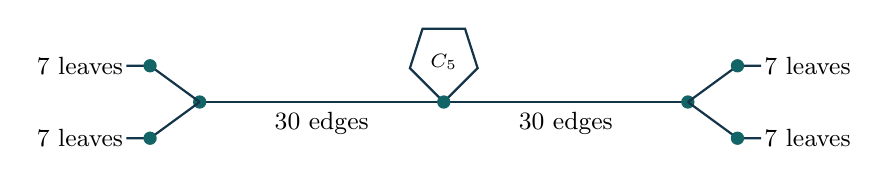
\begin{tikzpicture}[x=1cm,y=1cm, every node/.style={font=\small},edge/.style={draw=ink,thick},pt/.style={circle,fill=accent,inner sep=1.7pt}]
 \draw[edge] (0,0)--(3.1,0)--(6.2,0);
 \draw[edge] (3.1,0)--(2.67,.43)--(2.83,.93)--(3.37,.93)--(3.53,.43)--cycle;
 \node[font=\scriptsize] at (3.1,.51) {$C_5$};
 \node[below] at (1.55,0) {30 edges}; \node[below] at (4.65,0) {30 edges};
 \foreach \x/\q in {0/-1,6.2/1}{
  \node[pt] at (\x,0) {};
  \foreach \y in {-0.46,0.46}{
   \draw[edge] (\x,0)--({\x+\q*0.63},\y)--({\x+\q*0.93},\y);
   \node[pt] at ({\x+\q*0.63},\y) {};
   \node at ({\x+\q*1.52},\y) {7 leaves};
  }}
 \node[pt] at (3.1,0) {};
\end{tikzpicture}
\par\small The 97-vertex witness. Each of the four branch vertices has seven pendant neighbors.
\end{center}

For the finite witness take $(L,t,g)=(60,7,5)$. There are 28 leaves, 62 vertices of degree two, two of degree three, one of degree four and four of degree eight, giving the stated inverse degree. For a hand-check of the mode put $H(x)=\sum_{d\ge1}h_dx^d$ where $h_d$ counts unordered pairs at distance $d$. Set $B=2x+14x^2$, $C=2x+2x^2$, $E=16x+57x^2+14x^3+49x^4$. The first two polynomials count vertices other than the attachment root by depth in an endpoint branch pair and in the pentagon, respectively. $E$ counts unordered pairs within one rooted endpoint branch pair, including its root. Partitioning by the two attachment positions yields
\[
\begin{split}
 H(x)={}&\sum_{d=1}^{60}(61-d)x^d
  +2B\sum_{d=1}^{60}x^d+2C\sum_{d=1}^{30}x^d\\
 &+B^2x^{60}+2BCx^{30}+2E+5x+5x^2 .
\end{split}
\]
Its coefficients at $1,2,3,4,64$ are $97,186,126,195,196$. For $5\le d\le31$ they are $101-d$, at $32,33,34$ they are $73,124,115$, for $35\le d\le61$ they are $93-d$, and at $62,63$ they are $32,56$. Hence $64>725/12$ is uniquely modal. Counting both orientations and including the diagonal in the distance matrix gives the same unique mode.

For sharpness take $t\to\infty$ and $L=2\lfloor t^{3/2}/2\rfloor$. For large $t$ the diameter is $D=L+4$. The $4t^2$ cross-end leaf pairs have distance $D$. The other leaf pairs have distance two or four, with counts $4\binom t2$ and $2t^2$. At any fixed distance, the pairs meeting the connector path contribute $O_g(L+t)$: each vertex outside this path has at most two connector vertices at that distance, and pairs on the path itself contribute at most $L$. Pairs outside the connector meeting any of the $g-1$ nonroot cycle vertices or four parents contribute $O_g(t+1)$. Thus $D$ is uniquely modal for large $t$, since $L=o(t^2)$. Degree counting gives $J=L/2+4t+O_g(1)$ and $m/J\to2$. In the reverse direction a unicyclic graph on $n$ vertices has degree sum $2n$, so Cauchy--Schwarz gives $J\ge n/2$. Consequently $m\le n-1<2J$. This lower bound for $J$ also appears in Li and Shi's survey of the diameter and inverse degree.\footnote{X.~Li and Y.~Shi, \href{https://cfc.nankai.edu.cn/_upload/article/files/df/71/c19cfafd423ba2120480295ecad0/f08970b4-64b5-4620-9daf-a3f33905eeaa.pdf}{On the diameter and inverse degree}, \emph{Ars Combin.} 101 (2011), 481--487, Theorem~4 and its cited source.}
\end{proof}

\paragraph{The tie and independent-set choices in entries 92 and 95.}
The catalogue records Staton's odd-cycle counterexamples to a reading of 92 requiring a largest mode and a maximum independent set, and the tied example $C_9$ of Favaron, Mah\'eo and Sacl\'e for 95 (p.~44). The construction above removes both restrictions simultaneously, even on trees. Omit the cycle from $G(L,t,g)$; the same counting proof gives $m=L+4$ uniquely and $n=L+4t+5$. For a maximal independent set $S$ the coordinate of $v$ is $c_S(v)=|N(v)\cap S|$. It vanishes exactly on $S$. Every vertex covers at most three connector vertices in its closed neighborhood. Since $S$ dominates, $|S|\ge (L+1)/3$. Hence the right-hand side of 92 satisfies
\[
 \sum_{c_S(v)>0}\frac{1}{c_S(v)}\le n-|S|\le \tfrac23 L+O(t)<m
\]
for \emph{every} maximal $S$ when $t$ is large. For 95, alternate edges of the connector give a matching of size at least $L/2$. An independent set omits at least one endpoint from each matched edge, giving $\alpha\le n-L/2$. The residue theorem yields $\operatorname{res}(G)\le\alpha\le L/2+O(t)<m$.\footnote{O.~Favaron, M.~Mah\'eo and J.-F.~Sacl\'e, \href{https://doi.org/10.1002/jgt.3190150107}{On the residue of a graph}, \emph{J. Graph Theory} 15 (1991), 39--64.} Both deficits grow without bound. These are strengthenings of previously recorded refutations.

\paragraph{Positive subcase of the mean-distance claim 117R.}
Every connected graph with $e$ edges and $n\ge2$ vertices satisfies
\[
 \mu\le\frac{n+1}{3},\qquad J\ge\frac{n^2}{2e}.
\]
For the first bound pass to a spanning tree. When deleting a leaf from a tree of order $j$, at most $j(j-1)/2$ is lost from its unordered distance sum: the $i$th smallest positive distance from the leaf is at most $i$. Summing over $j$ and dividing by $\binom n2$ gives the first bound. Cauchy--Schwarz gives the second. Thus 117R holds whenever $2e(n+1)\le3n^2$. It holds in particular for every cactus of girth at least five. Indeed, rooting its block decomposition shows that each of its $b$ cycle blocks contributes at least four previously unseen vertices, while all other blocks are bridges, so $4b\le n-1$ and $e=n-1+b\le5(n-1)/4$. This proves 117R throughout the unicyclic class used in Theorem~\ref{thm:118}. The unrestricted girth-five mean-distance claim is left open here.

\section{A diameter bound for inverse temperatures (87)}\label{sec:87inverse}
The catalogue asks in entry 87 (p.~43) whether the variance of the distance matrix is at most the sum of reciprocal vertex temperatures. Its definition of temperature (entry $-1$) is $\theta_v=d(v)/(n-d(v))$. Thus the sum is $J_{\theta}=nJ-n$. The following bound also controls the population variance under any probability distribution on vertex pairs.
\begin{theorem}\label{thm:temperature}
In every connected graph of order $n\ge2$ and diameter $D$,
\[
 J_{\theta}\ \ge\ \frac{D^2}{4}+\frac{(D-2)^2}{12}+\frac1{n-1}.
\]
In particular 87 holds strictly, under either convention for including the diagonal of the distance matrix.
\end{theorem}
\begin{proof}
Split the vertices of a diametral path into three sets according to their positions modulo three. Within each set $S$ the vertices are pairwise at distance at least three. Their open neighborhoods are disjoint and avoid $S$. If $k=|S|>0$, then $\sum_{v\in S} d(v)\le n-k$, and Cauchy--Schwarz yields
\[
 \sum_{v\in S}\left(\frac{n}{d(v)}-1\right)
 \ge \frac{nk^2}{n-k}-k
 = k(k-1)+\frac{k^3}{n-k}
 \ge k(k-1)+\frac{k}{n-1}.
\]
The last bound holds for an empty class as well. Each of the other vertices contributes at least $1/(n-1)$. Write $k_1,k_2,k_3$ for the three class sizes. Since they sum to $D+1$, another application of Cauchy--Schwarz gives
\[
 J_{\theta}\ge\frac{n}{n-1}+\sum_{i=1}^3k_i(k_i-1)
 \ge\frac{n}{n-1}+\frac{(D+1)(D-2)}3,
\]
which rearranges to the claimed inequality. For a random distance $X\in[0,D]$, $X^2\le DX$, so $\operatorname{Var}(X)\le \mathbb EX(D-\mathbb EX)\le D^2/4$. This proves the strict form of the catalogued inequality.
\end{proof}


\section{Temperature deviation and average distance}
\label{sec:temp171}
Entries 170 and 171 of \emph{Written on the Wall} appear after the heading for triangle-free graphs. Entry 171 asks whether the population standard
deviation $\sigma_T$ of the vertex temperatures
$T_v=d_v/(n-d_v)$ satisfies $\mu\sigma_T\le n$
\cite[pp.~67--69]{wow}. Here $\mu$ is the mean distance over
distinct vertices of a connected simple graph. We prove the inequality and
determine the extremal graphs for all sufficiently large orders.

\begin{theorem}\label{thm:temp171}
Write $D$ for diameter and $\Delta$ for maximum degree. For $n\ge2$,
\[
 \mu\sigma_T\le D\sigma_T\le
 \frac{\Delta}{2}\left(1+\frac{1}{n-\Delta}\right)\le n-1.
\]
Let $U_n$ be the maximum of $\mu\sigma_T$ over graphs of order $n$. Then
\[
 U_n=Cn+C_0+O(1/n),\qquad
 C=\sqrt{y(1-y)}(1+y^2)=0.6828129\ldots,
\]
where $C_0=(y^2-y)\sqrt{y(1-y)}-(1+y^2)\sqrt{(1-y)/y}$ and $y$ is the unique root of $1-2y+5y^2-6y^3=0$ in $(1/2,3/4)$.
For all sufficiently large $n$, every maximizing graph is a complete
split graph $K_k\vee\overline K_{n-k}$, and $k=(1-y)n+O(1)$ on every
sequence of maximizers. In particular, for all such $n$,
\[
 U_n=\max_{1\le k\le n-2}
 (q-1)\sqrt{k/q}\left(1+\frac{q(q-1)}{n(n-1)}\right),
 \qquad q=n-k .
\]
\end{theorem}
\begin{proof}
A diameter path has $D+1$ vertices. A vertex off this path has at most
three neighbors on it, since two neighbors at least three steps apart
would shorten the path. A vertex on it has at most two neighbors on it.
In either case $\Delta\le n-D+1$. A variable with range in $[0,b]$
has standard deviation at most $b/2$, by computing its mean square
displacement from $b/2$. The temperatures belong to
$[0,\Delta/(n-\Delta)]$, which proves the finite bound.

Put $c=n-\Delta$. If $c\ge4$ the normalized product $\mu\sigma_T/n$
is at most $5/8$. If $2\le c\le3$, a maximum-degree vertex $v$ has
$c-1$ nonneighbors, all at distance at most $c$ from $v$ (after the first
step a shortest path from $v$ visits only nonneighbors). Averaging the
triangle inequality over pairs gives
\[
 \mu\le\frac2n\sum_{u}d(u,v)\le2+\frac{2(c-1)^2}{n}.
\]
Thus $\mu\sigma_T/n\le1/2+O(1/n)$ in these two cases.

It remains to treat graphs with a dominating vertex. Such graphs have
diameter at most two. Let $f(v)=1/(n-d_v)$, choose a uniform vertex
and put $A=\{v:n-d_v\le\sqrt n\}$ and $p=|A|/n$. Translation and
scaling give $\sigma_T/n=\operatorname{sd}(f)$. For
$Y=f\mathbf1_A$, the triangle inequality for centered random variables
gives $\left|\operatorname{sd}(f)-\operatorname{sd}(Y)\right|
\le n^{-1/2}$. Write $m=\mathbb EY$. Since $0\le Y\le1$ and $m\le p$,
\[
 \operatorname{Var}(Y)\le m(1-m)\le
 \begin{cases}p(1-p),&p\le1/2,\\1/4,&p\ge1/2.\end{cases}
\]
There are at most $n\sqrt n$ missing edges incident to $A$. All
nonedges have distance two. Consequently
$\mu\le1+(1-p)^2+O(n^{-1/2})$, uniformly in $p$.
For $p\ge1/2$ the normalized product is at most $5/8+O(n^{-1/2})$.
For $p\le1/2$ it is at most
$\sqrt{p(1-p)}(1+(1-p)^2)+O(n^{-1/2})$.
Writing $y=1-p$, differentiation shows that the sign of the derivative
of $\sqrt{y(1-y)}(1+y^2)$ is the sign of $1-2y+5y^2-6y^3$.
This polynomial is strictly decreasing on the real line and changes
sign between $1/2$ and $3/4$. Its maximum-value candidate exceeds $5/8$,
as witnessed by $y=2/3$. The complete split graph with $k$ universal
vertices and $q=n-k\ge2$ other vertices has
\[
 \mu=1+\frac{q(q-1)}{n(n-1)},\qquad
 \sigma_T=(q-1)\sqrt{k/q}.
\]
Taking $k$ to be the nearest integer to $(1-y)n$ attains
$Cn+O(1)$, establishing $U_n/n\to C$.

For any sequence of maximizing graphs the strict comparisons above force
a dominating vertex for all sufficiently large orders, and uniqueness
of the limiting maximum forces $p\to1-y\in(1/4,1/2)$. Also
$m\to1-y$: otherwise $\operatorname{Var}(Y)\le m(1-m)$ produces
a fixed loss on a subsequence, as $m\le p$ and $x(1-x)$ is strictly
increasing for $x<1/2$. At a nonuniversal vertex $f\le1/2$, so at most
$2n(p-m)=o(n)$ vertices in $A$ are nonuniversal. It follows that the
number $k$ of universal vertices satisfies $k/n\to1-y>1/4$.

Finally fix the $k$ universal vertices of any such maximizing graph and
form the complete split graph on the same partition. Write $a=k/n$,
$u=1/(n-k)$ and let $f_0$ be $1$ on the universal vertices and $u$
elsewhere. Its mean is $b=a+(1-a)u$. On nonuniversal vertices of the
original graph, $u\le f\le1/2$. Since $a\ge1/4$, the inequality
$1/2+u\le2b$ follows from $2a+(1-2a)u\ge1/2$
(the latter is linear in $u$ and holds at $u=0,1$). Hence
\[
 \operatorname{Var}(f)-\operatorname{Var}(f_0)
 =\mathbb E[(f-f_0)(f+f_0-2b)]-
       (\mathbb E[f-f_0])^2\le0 .
\]
Any additional edge among the nonuniversal vertices strictly decreases
the mean distance relative to the complete split graph and the latter
has positive deviation. Therefore every maximizer is complete split,
giving the discrete maximum in the statement.

To justify its expansion, for $z=q/n$ set $s(z)=\sqrt{z(1-z)}$,
$t(z)=\sqrt{(1-z)/z}$, and $h(z)=z^2-z$. The expression being maximized is exactly
\[
 n\Phi(z)+\Psi(z)+\frac{h(z)(s(z)-t(z))}{n-1},
 \quad
 \Phi=s(1+z^2),\qquad \Psi=hs-(1+z^2)t .
\]
The maximizing $z$ tends to $y$, where $\Phi''(y)<0$ by the
strictly negative derivative of the cubic above. On a fixed
neighborhood of $y$, all derivatives through order two are bounded
for $s,t,h,\Phi,\Psi$. Differences between the value at a maximizing
$z$ and at $z\pm1/n$ therefore imply $|\Phi'(z)|=O(1/n)$.
Consequently $z-y=O(1/n)$, and Taylor expansion gives
$U_n=n\Phi(y)+\Psi(y)+O(1/n)$.
\end{proof}

\paragraph{Two companion inequalities for triangle-free graphs.}
Write $m=|E|$ and $\omega$ for the clique number. Entry 170,
$\sigma_T\le m/\omega$, follows from $\sigma_T\le\Delta/2\le m/2$
when there is an edge, since $\omega=2$. The edgeless case gives
equality with zero. In particular it follows from the temperature
deviation estimate of Favaron, Mah\'eo and Sacl\'e
\cite[proof of conjecture 272]{temp171fms}.

For entry 217 use the gravity matrix of \cite[p.~52]{wow}.
For a pair of distinct vertices in the same component its entry is
$d_ud_v/[(n-1)d(u,v)]$; other entries are zero.
Let $\bar B$ be the mean above the diagonal, as in
\cite[glossary]{temp171bdf}. If $c=n-\Delta$, then
\[
 \bar B\le\frac{(2m)^2}{n(n-1)^2},\qquad
 \sigma_T\bar B\le\frac{2c\Delta^3}{n(n-1)^2}
 \le\frac{27n^3}{128(n-1)^2}< n\qquad(n\ge2).
\]
The first inequality follows by summing $d_ud_v$ over distinct ordered
pairs and bounding the sum by $(\sum d_v)^2$. For the second, the
neighborhood of a maximum-degree vertex is independent, so the other
$c$ vertices meet all edges and $m\le c\Delta$. Combine this with
$\sigma_T\le\Delta/(2c)$ and maximize $(1-x)x^3$ on $[0,1]$. This
proves entry 217 on its specified triangle-free class; when the
gravity mean vanishes the product form still makes sense.


\section{Simultaneous failure of five degree and distance inequalities}
\label{sec:syn-chains}
Write $J=\sum_v1/d_v$, $F=\max_j|\{v:d_v=j\}|$, $V$ for the population
variance of the degrees, and $m$ for the largest modal distance among
unordered pairs of distinct vertices. Let $Z$ count the vertices of
maximum degree. The degree and distance statistics in the original
conjectures 7, 8, 15, 16 and 17 can all be small on the very same graph.

\begin{theorem}\label{thm:syn-chain}
For every $A>0$ and integer $k_0\ge1$, there are graphs of arbitrarily
large order, of vertex connectivity at least $k_0$, for which
\[
 \min\{\mu,r\}> A\,(J+F+V+m+1).
\]
The graphs are unit interval graphs. For each fixed $A,k_0$ the examples
have uniformly bounded maximum degree and uniformly bounded modal distance.
In particular, no finite nonnegative coefficients $a,b,c,d$ and additive
constant $e$ give a universal upper bound
$\mu\le aI+bF+cV+dm+e$. The same conclusion holds for the radius, and
one may include $Z$ on the right since $Z\le F$.
\end{theorem}

\begin{proof}
Replace successive points of a path by nonempty cliques of prescribed
sizes. Join all vertices from consecutive cliques, and put no other
edges between cliques. Vertices from distinct layers at positions $i,j$
have distance $|i-j|$. Vertices in the same layer can be represented by
identical closed intervals of length one centered at the layer index.
This gives a unit interval representation. If every layer has at least
$k_0$ vertices, deleting fewer than $k_0$ leaves every layer nonempty
and the graph connected.

First consider any fixed list of $K\ge2$ positive layer sizes, repeated
$p$ times. Let $s_i$ be the size of layer $i$, with $1\le i\le pK$.
For $t\ge2$ the number $N_t$ of pairs at distance $t$ is
$\sum_{i=1}^{pK-t}s_i s_{i+t}$. For $t=1$ there are in addition the
pairs inside individual layers. Thus $N_{t+K}<N_t$ whenever
$1\le t<t+K\le pK-1$ since periodicity identifies the shorter sum
with a strict initial segment of the longer one. Hence $m\le K$.
The diameter is $pK-1$ and $r\ge(pK-1)/2$. For a pair of independent
uniform vertices, the indices $J,J'$ of their copies of the list are
independent and uniform on $\{0,\ldots,p-1\}$. Their distance differs
from $K|J-J'|$ by at most $K$. Since
$\mathbb E|J-J'|=(p^2-1)/(3p)$, and conditioning on distinct vertices
multiplies the mean by $n/(n-1)$, we obtain
\begin{equation}\label{eq:syn-chain-scale}
 \frac{\mu}{pK}\longrightarrow\frac13.
\end{equation}
The list fixes a uniform maximum-degree bound, and hence a variance
bound, independent of $p$.

It remains to choose the list so that both $J$ and $F$ grow slowly per
layer. Fix $\varepsilon>0$. Take a profile of $h$ layers with relative
sizes $w_i=q^{i-1}$, $1\le i\le h$, for integers $q\ge h\ge2$ with
$2/h<\varepsilon$. A copy of this profile at scale $j$ consists of
cliques of sizes $k_0 j w_i$. Except at its last layer, each vertex has
at least $q$ times its layer size in neighbors in the next layer. Thus
each of the first $h-1$ layers contributes at most $1/q$ to $J$. A
last layer of size $s$ has $s-1$ internal neighbors and at least one
external neighbor, so it costs at most one. Each profile contributes
at most $1+(h-1)/q\le2$ regardless of its neighbors.

Let $S=\sum_i w_i$. Select $M$ scales and a multiple $C$ of
$1,\ldots,M$. For each $1\le j\le M$, take $C/j$ consecutive profiles
all at scale $j$. Concatenate these $M$ runs to form the fixed list.
Writing $H_M=\sum_{j=1}^M1/j$, it has $K=hCH_M$ layers and yields
$J/(pK)\le2/h<\varepsilon$ after any number $p$ of repetitions.
Away from the very first and last layer of a run, a vertex in profile
position $i$ has degree
\[
 k_0 j(w_{i-1}+w_i+w_{i+1})-1,
\]
where profile subscripts are cyclic. At any fixed degree and fixed
position $i$, at most one scale $j$ can contribute by this formula.
That scale contributes at most $(C/j)k_0jw_i=Ck_0w_i$ vertices per list.
Hence every individual degree occurs at most $Ck_0 S$ times among all
these vertices per list. The first and last layers of all runs together
contain at most $B=2k_0w_h\sum_{j=1}^M j$ vertices per list, including
the layers at the ends of the whole path. Therefore
\[
 \frac{F}{pK}\le \frac{k_0 S+B/C}{hH_M}.
\]
First increase $M$ until the term $k_0S/(hH_M)$ is below
$\varepsilon/2$. Then choose the common multiple $C$ so large that
the remaining term is below $\varepsilon/2$. All layer sizes are now
fixed and at least $k_0$. Letting $p$ tend to infinity gives
\[
 \liminf\frac{\min\{\mu,r\}}{pK}\ge\frac13,
 \qquad \limsup\frac{J+F+V+m+1}{pK}\le2\varepsilon.
\]
Choosing $\varepsilon<1/(6A)$ proves the theorem.
\end{proof}

The repairs in 1988 are the particular choices $V+F$, $V+J$, and
$m+J$ as proposed upper bounds for $\mu$, and $V+F$, $Z+F$ for $r$.
Fixed coefficients cannot rescue even their sum. More generally, the
same proof allows an additional locally bounded function of $m,V$ and
maximum degree on the right: each such term is bounded for the fixed
list as $p$ increases. Bounded degree in this statement is uniform in
$p$ after the coefficient target is chosen. A single degree bound for
all targets would be impossible, since $J\ge n/\Delta$.

Erd\H{o}s, Pach and Spencer studied the extremal average distance at
fixed inverse-degree budget $J\le s$ and order $n$. For fixed $s\ge3$
they obtained order $\log n/\log\log n$ \cite{chain-eps}. Dankelmann, Swart and van den Berg sharpened the diameter bound \cite{eps-follow}. The present
construction lets $J$ grow along a repeated profile and simultaneously
controls $F,m,V$ and connectivity. For the two individual corrections
$V+J$ and $m+J$, a September 2026 public verification note already gives
clique-chain counterexamples \cite{chain-wow45}. Neither the earlier
counterexamples nor the use of a path of cliques carries a priority
claim here.


\subsection{The order of the largest violation}
For each $n\ge2$ let
\[
 Q_n=\max_{|V(G)|=n}\frac{\min\{\mu(G),r(G)\}}
             {1+J(G)+F(G)+V(G)+m(G)},
\]
where $G$ ranges over simple connected graphs. Using the minimum in the
numerator requires one example to defeat both proposed left-hand sides.

\begin{theorem}\label{thm:syn-chain-rate}
As $n\longrightarrow\infty$,
\[
 Q_n=\Theta\!\left(\frac{\log n}{\log\log n}\right).
\]
The same order holds when the numerator is replaced by $\mu$ alone, by
$r$ alone, or by the diameter $D$ alone.
\end{theorem}
\begin{proof}
Choose one end of a diametral geodesic as root. Write $x_i>0$ for the
breadth-first layer sizes, $0\le i<D+1=L$, and put zeros just outside
the layer interval. The degree of a vertex at level $i$ is smaller than
$x_{i-1}+x_i+x_{i+1}$. Define
\[
 \gamma_i=\max\{1,x_{i-1}/x_i,x_{i+1}/x_i\}.
\]
Then $J\ge\frac13\sum_i\gamma_i^{-1}$. Call a layer with
$\gamma_i=1$ a peak, and write $P$ for the number of peaks. In
particular $P\le3J$. At every other layer draw one arrow to a largest
adjacent layer. Layer sizes strictly increase along each arrow and every
arrow path terminates at a peak. A nonpeak has at most one incoming
arrow, since it sends an arrow to a strictly larger neighbor. A peak
receives at most two. The arrows thus partition into at most $2P$
monotone paths, the two paths at a peak possibly sharing that terminal
vertex. The sum of the logarithmic increases on each path is at most
$\log n$, by telescoping. Jensen's inequality now gives
\[
 \sum_i\log\gamma_i\le2P\log n\le6J\log n,
 \qquad J\ge\frac L3\exp\!\left(-\frac{6J\log n}{L}\right).
\]
In particular $x=L/J$ satisfies $x\log(x/3)\le6\log n$. Monotonicity for
$x\ge3$ gives $D/J=O(\log n/\log\log n)$, uniformly in $J$. This proves
all four upper bounds.

For the lower bound, put $h=\max\{j\ge4:j^{4j}\le n\}$, for all
sufficiently large $n$. Then $h=\Theta(\log n/\log\log n)$. A profile
has $h$ consecutive layers of sizes $s_i=h^i$, $0\le i<h$, of total
size $S=\sum_{i=0}^{h-1}h^i\le h^h$. Repeat it $p=\lfloor n/S\rfloor$
times, adding a final layer of size $n-pS$ when this is positive. Thus
$p\ge h^{3h}-1$. Consecutive layers are completely joined.

To control repeated degrees, give each layer of size $s$ the following
internal graph. For $u\ge1$ the graph on $1,\ldots,u$ with distinct
$x,y$ adjacent if $x+y\ge u+1$ has degrees
$x-\mathbf1_{\{2x\ge u+1\}}$. Each degree occurs at most twice. Join
two such graphs of orders $\lfloor s/2\rfloor$ and $\lceil s/2\rceil$
by all possible edges, omitting the empty part if $s=1$. This internal
graph has minimum degree at least $\lfloor s/2\rfloor$ and each degree
has multiplicity at most four. All vertices in a layer have the same
external degree.

The first $h-1$ layers in a profile each contribute at most $1/h$ to
$J$ by their larger successor. Its last layer, and the optional
remainder layer, each have external neighbors and hence contribute at
most $s/(1+\lfloor s/2\rfloor)\le2$. Therefore $J\le3p+2$.
For a fixed interior profile position $1\le i\le h-2$, full degrees
lie in the interval
\[
 [B_i,B_i+s_i-1],\qquad B_i=h^{i-1}+h^{i+1}.
\]
These intervals are disjoint as $i$ increases. Any degree therefore
occurs at most $4p$ times across these positions, at most $8p$ times
across the two end positions, and at most four times in the optional
remainder. Hence $F\le12p+4$. All layer sizes are at most $S$, so
$\Delta\le3S$ and $V\le9S^2=o(p)$.

Distinct layers still have distance equal to their separation. All
intralayer distances are one or two. For the periodic prefix, the
number of pairs from different layers at separation $t+h$ is strictly
less than at separation $t$ whenever $1\le t<t+h\le ph$. The extra
layer, when present, contributes its size times the size of the layer
$t$ positions earlier to separation $t$. Those contributions agree
at $t$ and $t+h$ by periodicity whenever both exist. Intralayer counts
can only increase the totals at $t=1,2$. Thus $m\le h$.

With probability $(pS/n)^2=1-o(1)$ two independent uniform vertices
lie in the periodic prefix. Conditional on that event, their profile
indices are uniform and independent; as in \eqref{eq:syn-chain-scale},
their mean distance is at least $h(p^2-1)/(3p)-h$. Conditioning on
distinct vertices only increases the overall mean. Consequently
$\mu\ge(1/3-o(1))hp$, while $r\ge(ph-1)/2$ by the diameter. The
denominator is $O(p)$ and the numerator is $\Omega(hp)$. This proves
the lower bound at every sufficiently large order.
\end{proof}
The examples in the quantitative lower bound use different internal
edges from the unit interval examples of Theorem~\ref{thm:syn-chain}.
The order statement specifies growth up to multiplicative constants.


\section{Exact finite certificates}\label{sec:finitecert}
For each vertex $u$ in each small witness, breadth-first search assigns distances $d(u,v)$ to its reachable vertices. Counting only $v>u$ gives a histogram $h_j$, which satisfies $\sum h_j=\binom n2$ and gives $W=\sum jh_j$. To bound $R$ without floating-point rounding, let $e_p$ count edges whose endpoint degrees have product $p$. At integer scale $Q$ take $a_p=\lfloor\sqrt{\lfloor Q^2/p\rfloor}\rfloor$. The lower and upper numerators for $QR$ are respectively $\sum e_pa_p$ and $\sum e_p(a_p+\mathbf1_{pa_p^2<Q^2})$.

\paragraph{The original items 3 and 5.} The 34-vertex graph in Section~\ref{sec:degree-data} gives $J=771/32$, $F=16$ and $R=2+4\sqrt2$. To check item~5, take the path $v_0,\ldots,v_{110}$, join $v_0$ to two new vertices, give each of these twelve leaves, and add twenty leaves at $v_{110}$. For this 157-vertex tree the five largest histogram entries, written $(j,h_j)$, are
\[
 (113,480),\quad(2,478),\quad(4,297),\quad(3,178),\quad(1,156).
\]
Here $W=576558$, $\mu=96093/2041$. The nonzero $(p,e_p)$ are
\[ (4,108),\quad(6,1),\quad(13,24),\quad(21,20),\quad(39,2),\quad(42,1).\] The integer bounds with $Q=10^{10}$ give $65.9035681063\le R\le65.9035681111$, hence $m=113>\mu+R$.

\paragraph{One graph violating both items.} In the construction of Theorem~\ref{thm:joint} take $k=5$, $s=2$, $L=2600$, and exactly $q=1000$ vertices of every degree type at each of the six terminals. The order is $14632$. The two largest histogram entries are $(2609,20000000)$ and $(14,16014618)$. Direct degree counts and the distance sum give
\[
 F=8610,\qquad J=\frac{20647619987}{2003001},\qquad
 \mu=\frac{96695782441}{107040396},\]
\[
 1671.158113563\le R\le1671.158131590 .
\]
Thus $m-\mu-R>34$ and $J-F-R>27$. The histogram can be reproduced by treating each terminal as a rooted graph with layer sizes $(1,s,sq)$. Write $N=sq$ and $E=qs(s+1)/2$. Within a single rooted graph the counts at distances $1,2,3$ are $s+E$, $N+\binom{s}{2}+\binom N2$, and $sN-E$. Regard each remaining skeleton vertex as a singleton at depth zero. For each unordered pair of distinct roots $u,v$ (including singleton roots), add the product of their layer sizes at depths $a,b$ to bin $a+d_{\rm tree}(u,v)+b$. These rules account for every unordered pair once.

\paragraph{Catalogue items 90 and 118R.} On the 250-vertex graph of Theorem~\ref{thm:ninety}, the census gives $W=1933683$ and $\mu=644561/10375$, with $B(S)=61$. A smaller witness uses the same four selected hubs at each endpoint of a path of length $100$. Select the path vertices of index $0,2\pmod 5$ and the three new hubs at each end. At each end take $23$ unselected vertices adjacent to the first three hubs and $23$ adjacent to all four. Its $199$ vertices have coordinate frequencies $(47,40,20,46,46)$ for coordinates $0$ through $4$. Its Wiener index $926820$ gives $\mu=102980/2189=47+97/2189$. On the 97-vertex girth-five graph of Theorem~\ref{thm:118}, the five largest histogram entries are $(64,196),(4,195),(2,186),(3,126),(33,124)$ and $J=725/12$.

\paragraph{Temperature extremizers at small orders.} For $n=3,4,5,6,7,8,9$, respectively, the $2,6,21,112,853,11117,261080$ connected unlabeled graphs each gave a unique maximizer up to isomorphism for $\mu\sigma_T$. In each case it was a complete split graph, with $1,1,1,1,2,2,2$ universal vertices, respectively. For reproducibility, enumerate the connected graph6 records at each order (for example with \texttt{geng -cq} followed by the order), compute $z_v=2520d_v/(n-d_v)$ and $W$ as above, and maximize the integer $W^2\bigl(n\sum_v z_v^2-(\sum_v z_v)^2\bigr)$. The common denominator in $(\mu\sigma_T)^2$ is $(2520n\binom n2)^2$. This is a finite check on Theorem~\ref{thm:temp171}.


\appendix
\section{A self-contained radius bound for the catalogue questions}
\label{sec:radius-certified}
Write $r$ for the vertex radius and give every edge length one. Let $\rho$
be the smallest possible maximum distance from a point on this metric
graph to its vertices. Rounding a center to a nearest vertex gives
$r-1/2\le\rho\le r$. A center can be chosen at a vertex or edge midpoint:
on an edge with coordinate $t\in[0,1]$, the distances to a vertex
are minima of two affine functions with integer intercepts and slopes
$1,-1$. Their ordering is constant on each open half-edge. The maximum
distance is therefore affine there as well, and its minimum occurs at a
half-edge endpoint.

The proof below condenses the degree-cut argument of VMRC~[161,171]
\cite{cat-rad,cat-harm}. We checked the two manuscripts at revision
\texttt{884d261108a87d22}; the corresponding degree-cut and harmonic
bounds are results of those earlier manuscripts.
\begin{theorem}\label{thm:radius-certified}
Every finite connected simple graph satisfies
$M:=\sum_{uv\in E}1/\max(d_u,d_v)\ge\rho$.
If its maximum degree is $\Delta\ge2$, then
\[
 H-r\ge\frac{\Delta-3}{2(\Delta+1)},\qquad
 R-r\ge\sqrt{\Delta}-\tfrac32.
\]
In particular the graphs with $H<r$ and those with $R<r$ are, in both
cases, precisely the even-order paths on at least four vertices.
\end{theorem}

\begin{proof}
\emph{Tree facts.} A tree of diameter $D$ has absolute radius $D/2$:
at the position $i$ on a diameter path, each branch has depth at most
$\min(i,D-i)$, so its vertices lie within $D/2$ of the midpoint.
The ends give the reverse inequality. If a connected $m$-vertex graph
has a vertex incident to $j\ge2$ edges, extend these edges to a spanning
tree. Each of its $j$ branches there contains a different leaf. A longest
path uses at most two leaves, so the tree has diameter at most $m-j+1$.
Consequently the graph satisfies $2r\le m-j+2$.

\emph{Reduction to a core and its leaves.} Suppose $M<\rho$, and minimize
first the cycle rank $|E|-|V|+1$, then $|E|$. Deleting a nonbridge
edge cannot lower $\rho$: distances between retained points can only
increase, and possible center locations are lost. Hence every such deletion
strictly increases $M$ by minimality. Deletion of a leaf on a support
$v$ of degree $d\ge2$ decreases $M$ by
\[
 \frac1d-\frac{b}{d(d-1)}\ge0,
\]
where $b$ counts its other neighbors of degree less than $d$.
The deleted edge contributes $1/d$ and exactly those $b$ edges
increase in weight. This deletion can lower $\rho$ by at most $1/2$.
Indeed, take a vertex or midpoint center $y$ of the remaining graph of
radius $r_0$. If its distance to $v$ is at most $r_0-1/2$, restoration
already costs at most $1/2$. Otherwise that distance equals $r_0$
by half-integrality; move $y$ half a unit toward $v$. This is possible
when the remaining graph has at least two vertices, and covers every
vertex within $r_0+1/2$. Stars and paths are checked directly, including
the singleton and single edge. In a remaining counterexample a support
of degree two has a nonleaf as its other neighbor; here the decrease
of $M$ is $1/2$, contradicting minimality. Two leaves on one support
are also impossible. After removing one, choose a center off the other
pendant interval: projection to the support can only reduce all other
distances, and the remaining leaf is now at distance one, at most
the radius since two vertices remain at distance two. Restoring the
deleted twin costs nothing.

For every $v$, at most one component of $G-v$ contains an edge.
Otherwise split those components into two sides $A,B$, each containing
an edge, and let $G_A$ keep $A\cup\{v\}$ with a new leaf for every
lost neighbor of $v$; define $G_B$ symmetrically. Both graphs preserve
the degree of $v$. Their cycle ranks sum to the original and each
has fewer edges, so both satisfy the desired absolute-radius bound.
Their added leaves together account for exactly one unit of index:
$M(G_A)+M(G_B)=M(G)+1$. Write $r_i=\rho(G_i)$ for $i=A,B$.
Each side has an artificial leaf and a retained neighbor of $v$, so
$r_i\ge1$ and we may project any center on an artificial pendant
interval to $v$. Choose such retained centers $y_i$ and write
$s_i=d(y_i,v)\le r_i-1$ by the distance to an artificial leaf.
On the path from $y_A$ through $v$ to $y_B$, use signed distance
$u\in[-s_A,s_B]$ from $v$. The two sides are covered with radii
$r_A+s_A+u$ and $r_B+s_B-u$, respectively. Their point of intersection,
if on the interval, has value at most $r_A+r_B-1$.
Otherwise the endpoint minimizing the larger function gives radius
$r_A$ or $r_B$, also at most $r_A+r_B-1$. Thus
$\rho(G)\le r_A+r_B-1\le M(G)$, a contradiction.

A tree of diameter at least four violates this cut-vertex property at
the third vertex of a diametral path. A smaller-diameter tree having
at most one leaf per support is a path. Hence our graph contains a
cycle. Choose a maximal induced two-connected subgraph $K$ containing
one. An outside component meeting $K$ at two distinct vertices would
give an ear between them: after deleting any one vertex the union of
the ear with $K$ stays connected. Thus each outside component has a
unique attachment. Removing that attachment shows that the component
contains no edge, since $K$ with one vertex removed is connected and
has an edge. The outside vertices are therefore leaves, with at most
one at each vertex of $K$. Every edge of $K$ is a nonbridge.

\emph{Counting the edges between degree classes.} All degrees in the
next calculation refer to $G$. At a core vertex $v$ let $p_v$ indicate an
attached leaf, $l_v$ count all strictly lower-degree neighbors and put
\[
 g_v=d_v(d_v-1),\qquad
 a_v=l_v/g_v,\qquad b_v=(d_v-l_v)/g_v .
\]
Deleting a core edge $uv$ with $d_u<d_v$ changes $M$ by $a_u-b_v$:
the remaining edges to lower-degree neighbors gain $1/g_u$ or $1/g_v$,
and the removed edge had weight $1/d_v$. For $d_u=d_v=d$ the change is
$(l_u+l_v-d+1)/(d(d-1))$. Both changes must be strictly positive.
If $l_u=0$, then $u$ has no leaf. A higher-degree neighbor violates the
first formula, and an equal-degree neighbor has $l_v\le d_v-1$,
violating the second. Thus $l_v\ge1$. All core degrees are at least
three, as a degree-two vertex has two nonleaf core neighbors. A core
vertex of smallest full degree must support a leaf. Removing all leaves
therefore gives a smaller graph $K$ and
\[
 0\le\delta:=M(G)-M(K)<\rho(G)-\rho(K)\le1 .
\]
The last bound uses the extension of any core center to all attached
leaves. If $\Delta=3$, then every core vertex has one lower-degree
neighbor, its leaf. Deleting any core edge gives change zero, a
contradiction. Hence $\Delta\ge4$.

For $3\le k<\Delta$, let $S$ be the core vertices of full degree at
most $k$, let $N_k$ count the core edges leaving $S$, and orient each
unequal-degree core edge from lower to higher. Denote by $I,F$ the
oriented edges inside and leaving $S$, and by $e_v$ the number of
equal-degree neighbors. At $v$ the indegree is $l_v-p_v$ and the
outdegree is $d_v-l_v-e_v$. Summing the identity
$(d_v-l_v)a_v=l_vb_v$ over $S$ gives
\[
 \sum_{v\in S}p_v b_v
  =\sum_{uv\in I}(a_u-b_v)+\sum_{uv\in F}a_u+\sum_{v\in S}e_v a_v.
\]
Delete only the leaves attached to $S$. The loss of $M$ is the left
side less $\sum_{uv\in Q}1/g_u$, where $Q$ consists of equal-degree
edges with a deleted leaf at each end. Indeed a strict edge changes its
weight only if its higher-degree end loses a leaf, in which case it gains
$1/g_v$ at that end. Its support loses $1/d_v$ and has $l_v-1$ such
core neighbors, leaving precisely $b_v$. An equal-degree edge gains
only when both ends lose leaves.
Each edge of $Q$ contributes $a_u+a_v\ge2/g_u$ to the final sum in the
display; the first sum is positive term by term. Deleting the remaining
leaves can only lower $M$ further. Thus
\[
 \delta\ge\sum_{uv\in F}a_u\ge \frac{N_k}{k(k-1)}.
\]

Write $m=|V(K)|$. On each edge the difference between the reciprocal
degree sum and twice its $M$-weight is $|1/d_u-1/d_v|$. Summing over
edges counts every vertex once in the reciprocal degree sum.
A core edge from degree $d$ to $e>d$ contributes
$\sum_{k=d}^{e-1}1/[k(k+1)]$. Subtract the leaf terms to obtain
\[
 m-2M=\sum_{k=3}^{\Delta-1}\frac{N_k}{k(k+1)}
          -\sum_{v\in K}\frac{p_v}{d_v}\le(\Delta-4)\delta\le\Delta-4.
\]
Here the removed leaf weights sum to at least $\delta$, as retained
edges only gain weight, and the first sum is at most
$\delta\sum_{k=3}^{\Delta-1}(k-1)/(k+1)\le(\Delta-3)\delta$.
A vertex of full degree $\Delta$ has at least $\Delta-1$ neighbors
in $K$. The spanning-tree construction gives a core tree of diameter
at most $m-\Delta+2$. Restoring the leaves increases its diameter by
at most two. Its midpoint yields $2\rho\le m-\Delta+4\le2M$, the
required contradiction.

\emph{Transfer to $H$ and $R$.} Put $n=|V(G)|$ and let an edge have
degrees $a\le b$. Its harmonic and modified weights are
$h=2/(a+b)$ and $m_e=1/b$. The identity
\[
 1/a+1/b=2h+(b/a-1)(h-m_e)
\]
gives $n\le2H+(\Delta-1)(H-M)$. For the ordinary index put
$q=1/\sqrt{ab}$. The analogous identity
$1/a+1/b=2q+(\sqrt{b/a}-1)(q-m_e)$ gives
$n\le2R+(\sqrt\Delta-1)(R-M)$. Using
$M\ge r-1/2$ and $n-2r\ge\Delta-2$ from the spanning-tree
construction yields the two stated bounds. Both are nonnegative for
$\Delta\ge3$. For $\Delta=2$ the graph is a path or a cycle.
For $n\ge3$,
$H(P_n)=(n-3)/2+4/3$, $R(P_n)=(n-3)/2+\sqrt2$ and
$H(C_n)=R(C_n)=n/2$, whereas both graph families have radius
$\lfloor n/2\rfloor$. The one-vertex and two-vertex graphs satisfy
$H=R=r$, completing the classification.
\end{proof}


\paragraph{The two original radius questions.} On an even path of order $n\ge4$ the deficit $r-R=3/2-\sqrt2<1$. On every other connected graph $R\ge r$ by the theorem, so $r\le R+1$ holds throughout. As $\mu\ge1$ this gives $r\le R+\mu$. In fact $R+\mu-r\ge1$: on the exceptional paths use $\mu=(n+1)/3$; elsewhere use $R\ge r$ and $\mu\ge1$. Equality requires $\mu=1$ in the latter case, hence completeness, and $R(K_n)=n/2$ shows that equality holds precisely on $K_2$.

\section{The mass-deletion proof for the original item 13}\label{sec:mass}
This appendix follows the proof audit of VMRC [226] and [227] \cite{audited,mass-audit}. To keep the degree multiplicity $F$ distinct from a quadratic optimization, write its optimal value as $\mathcal E$. Put $K(x,x)=2$, $K(x,y)=\dist(x,y)$ for $x\ne y$, and $\mathcal E(G)=\max_{p}p^{\mathsf T}Kp$, where $p$ ranges over the probability simplex. The maximum exists by compactness. We prove the manuscript's main estimate
\begin{equation} \mathcal E(G)\le M(G)+1.\label{weighted}\tag{W}\end{equation}
For every $G$ in scope, $M\ge1$: the edges at a maximum-degree vertex contribute exactly one.
\subsection{The possible shape of a counterexample}
Suppose a graph violates \eqref{weighted}. Choose one minimizing first its order and then its size, and fix a maximizing vector $p$. A connected proper subgraph $J$ of order at least two containing the support of any maximizing vector must have $M(J)>M(G)$. Indeed the distances of its remaining pairs can only increase, and minimality gives $\mathcal E(J)\le M(J)+1$. In particular
\begin{equation}
 M(G-e)>M(G)\quad\text{for every edge on a cycle.}\label{supportive}
\end{equation}
A star has $\mathcal E\le2=M+1$. In a double star write $a,b$ for the masses on the two sets of leaves. Only pairs from opposite leaf sets have kernel entry above two, so $\mathcal E\le2+2ab\le5/2$. The smaller number $l\ge1$ of leaves at a centre gives $M=1+l/(l+1)\ge3/2$.

For a vertex of degree at least two set $g_v=d_v(d_v-1)$ and let $\ell_v$ count its strictly lower-degree neighbours. Removing a leaf at $v$ decreases $M$ by
\begin{equation}
 b_v=(d_v-\ell_v)/g_v\ge0.\label{bleaf}
\end{equation}
The lost edge weighs $1/d_v$, and each of the other $\ell_v-1$ edges to a lower neighbour gains $1/g_v$. Thus a leaf in a minimal counterexample has positive mass for every maximizer.

We detail the cut-vertex step, since the diagonal convention matters here. If a cut vertex $v$ separates two nontrivial components, partition $G-v=A\sqcup B$ without crossing edges and with each side containing such a component. On side $A$ retain $v$ and replace its $d_B$ neighbours across the cut by $d_B$ new leaves; construct $G_B$ symmetrically. These padded graphs have fewer vertices or, in case of a tie, fewer edges, because the discarded side contains an edge. Old degrees are preserved and the new leaves give $M(G_A)+M(G_B)=M(G)+1$. Project $A$ identically to $G_A$ and send $B\cup\{v\}$ to a single new leaf; use the symmetric projection for $G_B$. The two projected kernel values sum to at least $K(x,y)+2$ for each pair. For a pair in one side the second value is two. For opposite sides the two new terminal edges add two. For $v$ paired with another vertex the surplus is three, and for $(v,v)$ it is two. Taking expectations contradicts minimality. Hence at most one component of $G-v$ can be nontrivial.

Remove all leaves and denote the remaining graph by $J$. It is connected; the one- and two-vertex possibilities were covered above. A cut vertex of $J$ would leave two components of the original graph containing non-leaf vertices, each nontrivial, contrary to the preceding paragraph. Thus $J$ is two-connected of order $h\ge3$. Two leaves at the same site have identical rows on the other vertices, and their $2\times2$ kernel is constant. Merging their masses would give a zero-mass leaf. Consequently each site $v$ in $J$ has at most one leaf $v'$. Call it \emph{loaded} when it has one, and set $\epsilon_v=1$ there and $0$ elsewhere. All core edges obey \eqref{supportive}. Moving the entire mass $t=p_v$ of a loaded site to its leaf increases the objective by $2t(1-t)$, because all other distances go up by one and the diagonal is two. The case $t=1$ gives $\mathcal E=2$. Thus $p_v=0$ at every loaded site.
\subsection{Degree restrictions and local deletion}
Put $a_v=\ell_v/g_v$, and use \eqref{bleaf} to define $b_v$ at every site. Deleting a core edge $uv$ gains $1/g_u$ on each surviving lower edge at $u$, and similarly at $v$, and loses its original weight. Hence \eqref{supportive} gives
\[
 d_u<d_v\Longrightarrow a_u>b_v,\qquad
 d_u=d_v\Longrightarrow a_u\ge b_v,\quad a_v\ge b_u .
\]
In the equal-degree case the strict inequality in the count is $\ell_u+\ell_v>d_u-1$, so the weak bounds follow by integrality. A site with no lower neighbour would contradict the first relation on a rising edge, or force $b_v=0$ on an equal edge where $u$ itself is not lower. A minimum-degree site therefore has a leaf and at least two core neighbours. Every site has total degree at least three. Every degree-three site is loaded, has exactly two core neighbours, and both have degree at least four by the equal-degree condition. This also rules out $h=3$.

Delete a site and its leaf if present, and denote the decrease of $M$ by $X_v$. The remaining graph is connected and has at least two vertices. Define
\[
 \beta_v=\epsilon_v b_v,\qquad \xi_v=\max(0,X_v,\beta_v).
\]
Every survivor edge can only grow in weight, while removed edges have total weight at most one. Thus $X_v\le1$. We need the following sharper bound.
\begin{lemma}\label{local}
At each site $0\le\beta_v\le\min(\xi_v,1/3)$ and $\xi_v+\beta_v\le1$.
\end{lemma}
\begin{proof}
Only a loaded site needs attention. Set $d=d_v$, $g=d(d-1)$, and let $l,e,u$ count its lower, equal and higher core neighbours. Then $l+e+u=d-1$ and $b_v=(e+u)/g\le1/d$. For a core neighbour $w$, its contribution to $X_v$ after subtracting survivor gains on its lower edges is $b_w$ if $d_w>d$, $b_w-1/g$ if $d_w=d$, and $1/d-a_w$ if $d_w<d$. If two equal-degree neighbours of $v$ are adjacent, the edge between them also gains, requiring a further subtraction. Dropping these nonnegative corrections gives an upper bound. The three preceding contributions are at most $a_v$, $a_v-1/g$ and $1/d-b_v$, respectively. Including the leaf edge gives
\[
 g X_v\le(d-1)+u(l+1)+el+l(d-1-e-u)=(l+1)(d-1)+u.
\]
Adding $gb_v=e+u$ leaves a shortfall from $g$ of $(d-2)e+(d-3)u\ge0$. Thus $X_v+b_v\le1$ and $2b_v\le2/3$, proving the claim.
\end{proof}
\subsection{The probability constraint}
For $u\in\supp p$, a one-sided transfer of mass from $u$ to any $z$ shows $(Kp)_u\ge(Kp)_z$. Averaging on the support yields $(Kp)_u=\mathcal E(G)$. Suppose $S$ is a set whose deletion leaves a connected graph of order at least two, and only $u\in S$ may have positive mass. Set $t=p_u$, $x=M(G)-M(G-S)$ and $\mathcal E=\mathcal E(G)$. If $t=0$, then $x<0$ by the subgraph argument. For $0<t<1$, renormalize the surviving vector by $1-t$. The kernels of surviving pairs can only rise and $\sum_{z\ne u}p_z\dist(u,z)=\mathcal E-2t$, whence
\[
 (1-2t)\mathcal E\le (1-t)^2(M+1-x)-2t^2 .
\]
For $0<t<1/2$, using $\mathcal E>M+1$ on the left gives $(1-t)^2x<(M-1)t^2$.

To justify the other half of the mass range, $M\ge2$ here: order the sites by decreasing degree and charge each edge to its first endpoint, putting leaves last. The first four sites contribute at least $\sum_{i=1}^4(1-(i-1)/3)=2$. Write $y=\sqrt{M-1}\ge1$ and $\theta(s)=\sqrt s/(y+\sqrt s)$. If $0<x\le1$, the last inequality gives $t>\theta(x)$ when $t<1/2$, and $\theta(x)\le1/2\le t$ otherwise. An unloaded site supplies mass for the deletion $\{v\}$. A loaded site supplies the same leaf mass for each of $\{v'\}$ and $\{v,v'\}$ because $p_v=0$. Summing these lower bounds over distinct masses yields
\begin{equation}
 \Theta:=\sum_{v\in V(J)}\theta(\xi_v)\le1.\label{budget}
\end{equation}

\subsection{Closing the weighted inequality}\label{sec:hand}
\begin{lemma}\label{saved}
Let $l_v$ count the lower \emph{core} neighbours of $v$, and $M_0$ be the weight of the core edges. Then
\[
 \sum_v X_v\ \ge\ M_0+\sum_{v\ \mathrm{loaded}}\frac{l_v}{g_v},
 \qquad M\le\sum_v(\xi_v+\beta_v).
\]
\end{lemma}
\begin{proof}
Sum the weight removed under site deletions. It is $2M_0+\sum_{v\ \mathrm{loaded}}1/d_v$ before the gains of surviving edges are subtracted. Each leaf edge at $w$ gains $1/g_w$ exactly $d_w-1$ times. For a core edge $uw$ with $d_u<d_w$, the gain $1/g_w$ occurs exactly when a core neighbour of $w$ other than $u$ is deleted. This is $d_w-1-\epsilon_w$ times, giving total $1/d_w-\epsilon_w/g_w$. On an equal-degree edge of degree $d$, gains occur only when a common neighbour is deleted, at most $d-1$ times, for total at most $1/d$. Subtract these gains. The unequal-degree term saves $1/g_w$ once for each lower core neighbour of a loaded $w$. Finally $1/d_v-l_v/g_v=b_v$ on a loaded site, since $\ell_v=l_v+1$. Adding the leaf weights to $M_0$ and using $X_v\le\xi_v$ proves the second claim.
\end{proof}
For a site with $x=\xi_v>0$, $b=\beta_v$, Lemma~\ref{local} gives $b\le x\le1-b$. The function $\sqrt{x}+b/\sqrt{x}$ is increasing on $x\ge b$, so
\[
 \frac{x+b}{\theta(x)}
   =(x+b)+y\bigl(\sqrt{x}+b/\sqrt{x}\bigr)
   \le1+\frac{y}{\sqrt{1-b}}\le1+\sqrt{3/2}\,y .
\]
At $x=0$ both summands in $x+b$ vanish. Lemma~\ref{saved} and \eqref{budget} now force $1+y^2=M\le1+\sqrt{3/2}\,y$, or
\begin{equation}M\le 5/2.\label{fivehalf}\end{equation}
\begin{lemma} If $h\ge5$, every surviving decorated core has $M>5/2$.\end{lemma}
\begin{proof}
Let $r$ be the number of sites of degree at least four. If some sites have degree three, each has two distinct higher neighbours, so $r\ge2$. For $2\le r\le4$, charge edges at the first endpoint in decreasing order. The first $r$ sites contribute at least $r-\binom r2/4$. Each remaining site contributes a separate leaf edge of weight $1/3$. At $h=5$ these lower bounds for $r=2,3,4$ are $11/4,35/12,17/6$. They increase with $h$. If $r\ge5$, the first five sites alone contribute at least $5-10/4=5/2$. For $h>5$ choose the last site in this ordering. Its lower neighbour must be a leaf, and that edge was uncounted. For $h=5$, a missing pair among the five gives strictness in counting earlier neighbours. If the core is $K_5$, an unloaded site would have degree four and no lower neighbour. All sites are therefore loaded and $M=3$.
\end{proof}
It remains to handle $h=4$. Every site has core degree at least two, so the missing pairs of $J$ form a matching. Project a leaf to its site and each site to itself, and write $q$ for the resulting masses. For independent samples $x,y$ from $p$, $K(x,y)\le2+\dist_J(\pi x,\pi y)$ even on the diagonal. Missing pairs have distance two, and hence
\[
 \mathbb E_q\dist_J
 =1-\sum_i q_i^2+2\sum_{ij\ \mathrm{missing}}q_iq_j\le1
\]
by $2q_iq_j\le q_i^2+q_j^2$ on disjoint pairs. Thus $\mathcal E\le3\le M+1$. This contradicts minimality in the last possible case and proves \eqref{weighted}. In particular, no external computation is needed for this proof of the weighted theorem.



\subsection{Returning to the ordinary mean}
Uniform mass on all vertices and equal mass on two diameter endpoints in \eqref{weighted} give, respectively,
\begin{align}
 M&\ge\frac{(n-1)\mu-(n-2)}n ,\label{uniform}\\
 M&\ge D/2.\label{diameter}
\end{align}
The second is the published theorem of Dvo\v{r}\'ak, Lidick\'y and \v{S}krekovski \cite{dls}. For the first, the coefficient $(n-1)/n$ comes from drawing with replacement; the diagonal contributes $2/n$. For an edge with endpoint degrees $a\le b$ the identity
\[
 (a^{-1/2}-b^{-1/2})^2=(\sqrt{b/a}-1)((ab)^{-1/2}-b^{-1})
\]
and summation over edges, with $r=\sqrt\Delta$, give
\begin{equation}
 (r+1)R\ge n+(r-1)M.\label{randicbridge}
\end{equation}
We now deduce $R>\mu$ for $n\ge3$. For $n\ge5$ a hypothetical $R\le\mu$ requires
\[
 \mu\ge\frac{n^2-(r-1)(n-2)}{2n+r-1}.
\]
The right-hand side decreases in $r$. At $r=\sqrt{n-1}$ it is at least $(n+1)/3$ because the numerator of the squared comparison factors as $(n-5)(n-2)(n^2-5n+5)$. The classical path bound $\mu\le(n+1)/3$ has equality only on $P_n$ \cite{ejs}. One sees this by passing to a spanning tree, deleting a leaf and bounding its transmission by $1+\cdots+(n-1)$. An extra edge strictly shortens a pair, and equality in the leaf bound forces a path. Equality throughout would require both $G=P_5$ and $\Delta=4$, which is impossible. For $n=3,4$ the degree comparison with $M\ge1$ gives $R\ge(n+r-1)/(r+1)\ge\sqrt{n-1}>(n+1)/3$, since $r=\sqrt\Delta\le\sqrt{n-1}$. At $n=2$ the only graph is $K_2$ and gives equality. This completes the proof of the original item 13 for all orders.
\begin{thebibliography}{99}
\bibitem{chain-wow45} AI Village, \emph{WOW-I 4 and 5: two repairs of the inverse-degree inequality}, public verification notes and source code, 3 September 2026, commit \texttt{42dc4b3}. \href{https://gitlab.com/ai-village-agents/village/graffiti-verification/-/blob/main/verify/notes_wow1_4_and_5_2026-09-03.md}{Repository notes}.
\bibitem{chung} F. R. K. Chung, The average distance and the independence number, \emph{J. Graph Theory} \textbf{12} (1988), 229--235. \doi{10.1002/jgt.3190120213}.
\bibitem{temp171fms} O. Favaron, M. Mah\'eo, and J.-F. Sacl\'e,
The Randi\'c index and other Graffiti parameters of graphs,
\emph{MATCH Commun. Math. Comput. Chem.} 47 (2003), 7--23.
\url{https://match.pmf.kg.ac.rs/electronic_versions/Match47/match47_7-23.pdf}.
\bibitem{eps-follow} P. Dankelmann, H. C. Swart and P. van den Berg, Diameter and inverse degree, \emph{Discrete Math.} \textbf{308} (2008), 670--673.
\bibitem{chain-eps} P. Erd\H{o}s, J. Pach and J. Spencer, On the mean distance between points of a graph, \emph{Congressus Numerantium} \textbf{64} (1988), 121--124. \href{https://www.renyi.hu/~p_erdos/1988-23.pdf}{Author archive}.
\bibitem{ejs} R. C. Entringer, D. E. Jackson and D. A. Snyder, Distance in graphs, \emph{Czechoslovak Math. J.} \textbf{26} (1976), 283--296. \doi{10.21136/CMJ.1976.101401}.
\bibitem{wow} S. Fajtlowicz, \emph{Written on the Wall}, July 2004 electronic catalogue. \href{https://independencenumber.wordpress.com/wp-content/uploads/2012/08/wow-july2004.pdf}{Source text and numbering}.
\bibitem{faj} S. Fajtlowicz, On conjectures of Graffiti, \emph{Discrete Math.} \textbf{72} (1988), 113--118. Also in \emph{Ann. Discrete Math.} \textbf{38}. \doi{10.1016/0012-365X(88)90199-9}.
\bibitem{earlier-modes} Shaitetsu, \emph{Distance modes and extremal graph inequalities}, research manuscript, 21 November 2026, Sections 1--5. The original 157-vertex example is specified in full in Section~\ref{sec:finitecert} above.
\bibitem{temp171bdf} T.~L. Brewster, M.~J. Dinneen, and V. Faber,
A computational attack on the conjectures of Graffiti: New counterexamples and proofs,
\emph{Discrete Math.} 147 (1995), 35--55.
\url{https://www.cs.auckland.ac.nz/~mjd/graffiti/graffiti1.pdf}.
\bibitem{cat-rad} Verifiable Mathematical Reasoning Corpus, \emph{A proof of the Caporossi--Hansen conjecture on the Randi\'c index and graph radius}, manuscript [161], November 2026. \href{https://github.com/QEEDDD/Verifiable-Mathematical-Reasoning-Corpus/blob/884d261108a87d2229e5bcc273e5f4a607c771d2/\%5B161\%5D\%20Randic_Index_and_Vertex_Radius.tex}{Frozen source manuscript}.
\bibitem{cat-harm} Verifiable Mathematical Reasoning Corpus, \emph{Harmonic index and radius: a strengthening of the Caporossi--Hansen inequality}, manuscript [171], November 2026. \href{https://github.com/QEEDDD/Verifiable-Mathematical-Reasoning-Corpus/blob/884d261108a87d2229e5bcc273e5f4a607c771d2/\%5B171\%5D\%20Harmonic_Radius_Master_Theorem.tex}{Frozen source manuscript}.
\bibitem{audited} Verifiable Mathematical Reasoning Corpus, \emph{The Randi\'c index is at least the average distance}, manuscript [226], 20 November 2026. \href{https://github.com/QEEDDD/Verifiable-Mathematical-Reasoning-Corpus/blob/884d261108a87d2229e5bcc273e5f4a607c771d2/\%5B226\%5D\%20Fajtlowicz_Average_Distance_Proof.tex}{Archived source}.
\bibitem{mass-audit} Verifiable Mathematical Reasoning Corpus, \emph{A proof audit of Fajtlowicz's average-distance conjecture}, manuscript [227], 2026. \href{https://github.com/QEEDDD/Verifiable-Mathematical-Reasoning-Corpus/blob/884d261108a87d2229e5bcc273e5f4a607c771d2/\%5B227\%5D\%20Fajtlowicz_Proof_Audit.tex}{Archived source}.
\bibitem{degree-caro} Y. Caro and D. B. West, Repetition number of graphs, \emph{Electron. J. Combin.} \textbf{16} (2009), R7. \doi{10.37236/96}.
\bibitem{dls} Z. Dvo\v{r}\'ak, B. Lidick\'y and R. \v{S}krekovski, Randi\'c index and the diameter of a graph, \emph{European J. Combin.} \textbf{32} (2011), 434--442. \doi{10.1016/j.ejc.2010.12.002}.
\end{thebibliography}
\end{document}
